\section{FA 1.7 - 1 Zu- und Abwanderung - MC - BIFIE}

\begin{beispiel}[FA 1.7]{1} %PUNKTE DES BEISPIELS
In der untenstehenden Graphik wird das Wanderungssaldo -- das entspricht der Differenz von Zuwanderung und Abwanderung -- dargestellt. Zusätzlich werden ab dem Jahr 1995 Zu- und
Abwanderung durch Graphen von Funktionen dargestellt. Ab dem Jahre 2012 sind die angegebenen Zahlen als prognostische Werte zu interpretieren.

Angegeben wird jeweils die Anzahl derjenigen Personen, die bundesweit nach Österreich zu bzw. abgewandert sind.		


\begin{center}
\includegraphics[width=0.6\textwidth]{../_database/Bilder/GrafikFA171.eps}
\end{center}\vspace{-1cm}
\begin{flushright}
\tiny{Quelle: Statistik Austria} \hspace{1cm}
\end{flushright}
%%\begin{figure}%
%\includegraphics[width=0.7\textwidth]{GrafikFA171}%
%%\caption{Quelle: Statistik Austria}%
%%\end{figure}

Kreuze die beiden zutreffenden Aussagen an!
\multiplechoice[5]{  %Anzahl der Antwortmoeglichkeiten, Standard: 5
				L1={Werden die Graphen der Funktionen "`Zuwanderung"' und "`Abwanderung"' bis 1960 weitergezeichnet, verläuft der Graph der Zuwanderungsfunktion stets oberhalb des Graphen der Abwanderungsfunktion.},   %1. Antwortmoeglichkeit 
				L2={Es gibt Jahre, in denen sich die Zuwanderungs- und die Abwanderungszahlen um weniger als 5\,000 voneinander unterscheiden.},   %2. Antwortmoeglichkeit
				L3={Wird der Graph der Abwanderungsfunktion bis 1960 gezeichnet, verläuft er genau achtmal unterhalb der Nulltausenderlinie.},   %3. Antwortmoeglichkeit
				L4={Wenn die Graphen der Zuwanderungs- und der Abwanderungsfunktion über einen längeren Zeitraum parallel verlaufen, bleibt der Wanderungssaldo in diesem Zeitraum konstant.},   %4. Antwortmoeglichkeit
				L5={Ab 2020 wird eine lineare Abnahme der Abwanderungszahlen prognostiziert, d. h. die jährliche prozentuelle Abnahme der Abwanderungszahlen wird als konstant angenommen.},	 %5. Antwortmoeglichkeit
				L6={},	 %6. Antwortmoeglichkeit
				L7={},	 %7. Antwortmoeglichkeit
				L8={},	 %8. Antwortmoeglichkeit
				L9={},	 %9. Antwortmoeglichkeit
				%% LOESUNG: %%
				A1=2,  % 1. Antwort
				A2=4,	 % 2. Antwort
				A3=0,  % 3. Antwort
				A4=0,  % 4. Antwort
				A5=0,  % 5. Antwort
				}
\end{beispiel}